\documentclass{standalone}
\usepackage{tikz} % To generate the plot from csv
\usepackage{pgfplots}
\usepackage{pgfkeys}
\usepackage{mathrsfs}

\newenvironment{customlegend}[1][]{%
    \begingroup
    % inits/clears the lists (which might be populated from previous
    % axes):
    \csname pgfplots@init@cleared@structures\endcsname
    \pgfplotsset{#1}%
}{%
    % draws the legend:
    \csname pgfplots@createlegend\endcsname
    \endgroup
}%

% makes \addlegendimage available (typically only available within an axis environment):
\def\addlegendimage{\csname pgfplots@addlegendimage\endcsname}

% graph colors
\definecolor{blue}{rgb}{0.0, 0.0, 1.0}
\definecolor{red}{rgb}{1.0, 0.03, 0.0}
\definecolor{purple}{rgb}{0.54, 0.17, 0.89}
\definecolor{green}{rgb}{0.13, 0.55, 0.13}
	
\begin{document}
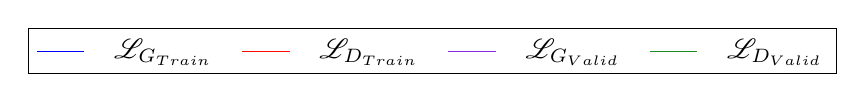
\begin{tikzpicture}
    \begin{customlegend}[
      legend columns=4,
      legend style={column sep=2ex},
      legend entries={$\mathscr{L}_{G_{Train}}$,$\mathscr{L}_{D_{Train}}$,$\mathscr{L}_{G_{Valid}}$,$\mathscr{L}_{D_{Valid}}$}
    ]
    \addlegendimage{blue}
    \addlegendimage{red}
    \addlegendimage{purple}
    \addlegendimage{green}
    \end{customlegend}
\end{tikzpicture}
\end{document}